\chapter{Código}
\section{Funciones Auxiliares}
Antes de explicar las funciones pedidas, comentaremos brevemente las funciones auxiliares que hemos utilizado: 
\subsubsection{char** reservarEspacio(int)}
Esta función se encarga de reservar el espacio necesario para que nuestro array de soluciones tenga el tamaño justo, y cada elemento de dicho array pueda almacenar cualquier String que se introduzca por la entrada.
\subsubsection{void liberarEspacio(char**,int)}
Esta función se encarga de liberar la memoria dinámica tras su uso. Recibe el array de punteros donde se guarda nuestra solucion y le aplica $free$ a todos sus elementos.
\subsubsection{void imprimir-normal(char**,int)}
Método muy simple que imprime todos los Strings almacenados hasta que llega al límite.
\subsubsection{void imprimirTail (char**,int,int)}
Método para imprimir la solución de la función $tail$, necesaria debido a que ésta tiene que imprimir la solución empezando por una posición que no tiene por qué ser la primera.
Así, esta función recibirá como parámetros $solución$, j (la última posición en la que se guardó el parámetro de entrada en el array) +1, y N, que es el tamaño del array solución. Para recorrer el array, solo es necesario un bucle que vaya de i hasta N, y que en cada iteración imprima $solución[(j+i)\%N]$.
\subsubsection{int longitud (char**)}
Devuelve el número de elementos no nulos que contiene el array.
\subsubsection{int menor (char**,int)}
Método que indicará en la función longlines dónde tiene que insertarse el elemento entrada. Para ello obtendrá el tamaño del String entrada, e irá comparando los tamaños de los Strings ya guardados en solución hasta encontrar uno que no lo supere.
\subsubsection{void insertar (char**,char*,int,int)}
Método principal de la función longLines. Se encarga de mover los elementos del array hacia la derecha a partir de la posición donde se situará  del array, y a continuación inserta el elemento de entrada en su posición correcta. Para más información ver función longLines. 
\section{Función head}
La primera función a implementar es $int$ $head$ $(int$ $N)$, que deberá comportarse como \textit{head(1)} y devolver las N primeras lineas en la salida estándar recibidas por entrada estándar.
En esta, primero reservamos espacio en una variable $entrada_uno$, en el cual iremos guardando los parámetros introducidos por consola. Mediante un bucle de N iteraciones, cada vez que se introduce un string por la entrada estándar, esta se guardará en la variable $entrada_uno$, y se imprimirá por pantalla.
Cuando el bucle termina, se libera el espacio usado por la variable $entrada_uno$ y se finaliza la función.
%En esta, primero reservamos espacio en una variable $solución$ llamando a la función $reservarEspacio$, descrita anteriormente. Luego, mediante un bucle de N iteraciones, guardamos los parámetros que vayamos recibiendo por consola en la posición i de $solución$.
%Al terminar el bucle, llamamos a la función $imprimir-normal$, que lo que hará será recorrer la variable $solución$ imprimiendo por pantalla cada string guardado en cada posición del mismo.
\section{Función tail}
La segunda función a implementar es $int$ $tail$ $(int$ $N)$, que deberá comportarse como \textit{tail(1)} y devolver las N últimas lineas en la salida estándar recibidas por entrada estándar.
En esta función se repite el mismo método de reservar espacio. Cuando se ha reservado espacio en la variable $solución$, se pasa a guardar la información que se pase por entrada en esta variable. Para ello, se requerirá, a parte de la variable contador i, otra variable j auxiliar, que durante el bucle se actualizará a $j=i\%n$. Esto es debido a que hay que simular que la variable solución es un array estático que hace la función de una cola. Lo hemos hecho así para no malgastar espacio de manera innecesaria, como se hubiera hecho si hubiesemos reservado un espacio determinado, y luego hubiesemos leido las N últimas posiciones (además de poder pasar por entrada tantas líneas como se desee).
\begin{figure}[htb]
\begin{center}
\centering
  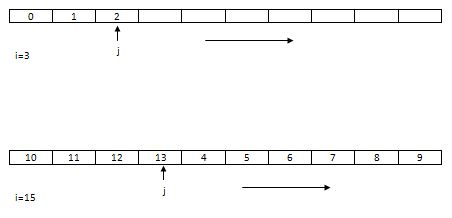
\includegraphics[width=0.8\textwidth]{./img_1}
  \caption{funcionamiento del Tail}
  \label{fig:Funcionamiento del Tail}
\end{center}
\end{figure} 

El bucle por lo tanto realiza iteraciones mientras $entrada != NULL$, y va guardando en la posición $j=i\%n$ de solución el parámetro $entrada$ recibido, y actualizando posteriormente la variable i (i++).
Por último, tras salir del bucle (CTRL+D) se procede a imprimir por pantalla el array $solución$ llamando a la función $imprimirTail$.
\section{Función longLines}
Por último, se nos pide implementar la función $int$ $longlines$ $(int$ $N)$, que mostrará las N líneas más largas de forma ordenada recibidas por la entrada estándar.
En esta función se vuelve a utilizar el método de reservar espacio para el array $solución$. Posteriormente, entramos un bucle que iterará mientras $entrada != NULL$ en el que se irán metiendo en $solución$:
\begin{itemize}
\item Todas las líneas recibidas por entrada estándar si el array posee menos de N elementos
\item O en el caso de que ya esté lleno, se meterá la línea recibida si es más larga que la línea más corta del array.
\end{itemize}
Siempre que se inserte un elemento en $solución$, se hará en el sitio que corresponda, desplazando los elementos que estén a su derecha un puesto hacia la derecha (eliminando el último en el caso de que el array esté lleno)
Este proceso se lleva acabo:
\begin{itemize}
\item Guardando en una variable auxiliar $tam_menor$ La longitud de la línea de menor longitud insertada en el array (situada en la posición $solución[n-1]$) actualizada al principio de cada iteración,
\item Una condición en la que solo entrará si se puede insertar $entrada$ en $solución$ (cuando esta es menor que la menor del array)
\item Y una función auxiliar llamada $insertar$ dentro de la condición anterior que recibirá el array $solución$, la variable $entrada$ y la posición en la que ha de ser insertada, para insertarla correctamente.
\end{itemize}
\begin{figure}[htb]
\begin{center}
\centering
  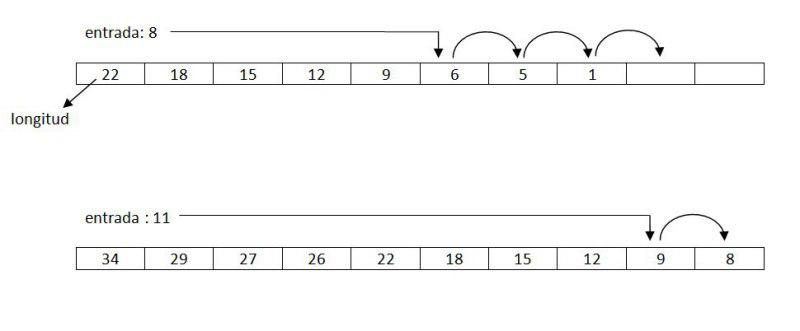
\includegraphics[width=0.8\textwidth]{./img_2}
  \caption{Funcionamiento del longLines}
  \label{fig:Funcionamiento del longLines}
\end{center}
\end{figure} 

La función auxiliar $insertar$, recorre de derecha a izquierda hasta la posición en la que ha de insertar $entrada$, situando el elemento $solución[i-1]$ en $solución[i]$. Cuando finaliza, solo le queda por insertar en la posición correspondiente el valor entrada.
Por último, una vez salido del bucle, solo queda imprimir por pantalla la lista solución llamando a la función $imprimir_normal$ explicada en la primera función (no es necesario crear una función imprimir específica para esta como en $tail$, puesto que el array ya viene ordenado y listo para ser impreso).
\section{Makefile}
Debido a lo tedioso que podría llegar a ser ir compilando el test.c y la librería, además de que se creaban archivos innecesarios (libreria.o y test.o ), decidimos crear un pequeño makefile que se encargaría de hacer todas estas compilaciones y posteriores borrados, facilitando enormemente nuestro trabajo.
\chapter{Comentarios personales}
\section{Problemas encontrados}
Como era la primera vez que trabajábamos con C, y estando acostumbrados a java, en un primer momento el manejo de punteros se nos hizo bastante complejo. Tuvimos en un principio varias dudas respecto al uso de memoria dinámica y el funcionamiento de la función $fgets$.
También pequeños detalles que aunque no muy graves, restaban calidad a nuestro código. La declaración de variables al principio del código o declarar las funciones que se van a invocar serían dos ejemplos de ello. \\
Por otra parte tuvimos que lidiar con la creación de un pequeño makefile que nos ahorrara mucho tiempo compilando los archivos.
\section{Posibles mejoras}
Tras ejecutar $valgrind --leak-check=full$, pudimos comprobar que perdíamos solo 39 bytes en fugas de memoria, y considerando que era nuestro primer contacto con punteros, no nos parece un número excesivo. Respecto a los algoritmos empleados, la función longLines podría tener un coste menor con un algoritmo clásico de ordenación, como burbuja o mergeSort, aunque nosotros decidimos hacer uno propio, obteniendo así un algoritmo probablemente "peor", pero mejorando y practicando nuestros conocimientos.